%----------------------------------------------------------------------------
\chapter{A Train Benchmark}
%----------------------------------------------------------------------------
Egy számítógép által elvégzendő felügyeleti, esetleg irányítási feladat elvégzéséhez általában elkészítünk egy modellt, ami a rendszer egy leírása. A modell a világ képzelt vagy valós elemeit és ezeknek a számunkra fontos tulajdonságait írja le. Egy valós modellezési folyamat során olyan komplex maga a valóság is, hogy képtelenség hiba nélkül elsőre előállítani a modellt. A hibák ellenőrzésére általában ki szoktak kötni kényszereket, melyek olyan megkötések, amik nem lehetséges eseteket zárnak ki. Egy valós fejlesztési folyamat során megalkotnak egy modellt, ami általában nem hibamentes, az előre meghatározott kényszerek sem teljesülnek rájuk. Utána minden fejlesztési szakaszban kijavítanak néhány hibát, majd újraellenőrzik a modellt és ezt ciklikusan folytatják addig, amíg minden kényszernek meg nem felel. Sok esetben ezzel párhuzamosan történik a modell bővítése is, ami újabb hibákat eredményez.

A modell elemeit minden esetben valamilyen adatbázisban tárolják. Mivel az adatokon végzett műveletek többségét támogatják elterjedt adatbázis-kezelő szoftverek, ezért többnyire a fejlesztési folyamatban egy ilyen szoftvert választanak. A Train Benchmark egy ilyen folyamat különböző adatbázis-kezelő szoftvereken való lefuttatását hasonlítja össze, ezzel szimulálva a valós fejlesztést és célja a szoftverek teljesítményének összehasonlítása.

\section{A modell felépítése}

A Train Benchmark egy vasúti pályának az elemeit, azok tulajdonságait használja fel egy valós probléma szimulálására. A modell osztályokból épül fel, amik meghatározzák az adott elemnek az általunk fontos tulajdonságok összességét, ezeket tároljuk. Ezek az osztályok a következők:
\begin{itemize}
	\item \emph{RailwayElement}: Minden osztály ennek az osztálynak a leszármazottja. Egyetlen közös tulajdonságot, az egyedi azonosítót tartalmazza.
	\item \emph{Semaphore}: Jelzi a vonatnak, hogy az adott útszakaszon áthaladhat-e. Az aktuális állapotát tároljuk. (A továbbiakban: szemafor)
	\item \emph{TrackElement}: A sípálya legkisebb számunkra fontos alkotóelemei, a \emph{Segment} és a \emph{Switch} ősosztálya.
	\item \emph{Segment}: Az útnak egy kisebb része, ami már megfigyelhető szenzorok által. A modellben szereplő tulajdonsága a hossza. (A továbbiakban: útszakasz)
	\item \emph{Switch}: Két útszakasz között helyezkedik el és meghatározza azt, hogy merre halad tovább a vonat, amikor ideér. (A továbbiakban váltó)
	\item \emph{Route}: Egy vasúti sínpár szakasza két szemafor között. útszakaszokból és váltókból áll össze. Azt tároljuk róla, hogy aktív-e, azaz, hogy az összes váltó olyan állásban van, hogy a vonat ezen az útvonalon halad végig. (A továbbiakban: út)
	\item \emph{Region}: Szenzorokat, útszakaszokat és váltókat magába foglaló konténer. (A továbbiakban régió)
	\item \emph{RailwayContainer}: Utakat és a régiókat tartalmazó konténer.
	\item \emph{Sensor}: A hozzá tartozó útszakaszokat, illetve váltókat monitorozza. (A továbbiakban: szenzor)
	\item \emph{SwitchPosition}: A váltó az úthoz mért relatív állását mutatja, azaz, hogy a váltónak merre kell állnia, hogy a szegmenseken végighaladó vonat az adott úton haladjon. 
\end{itemize}

\begin{figure}
	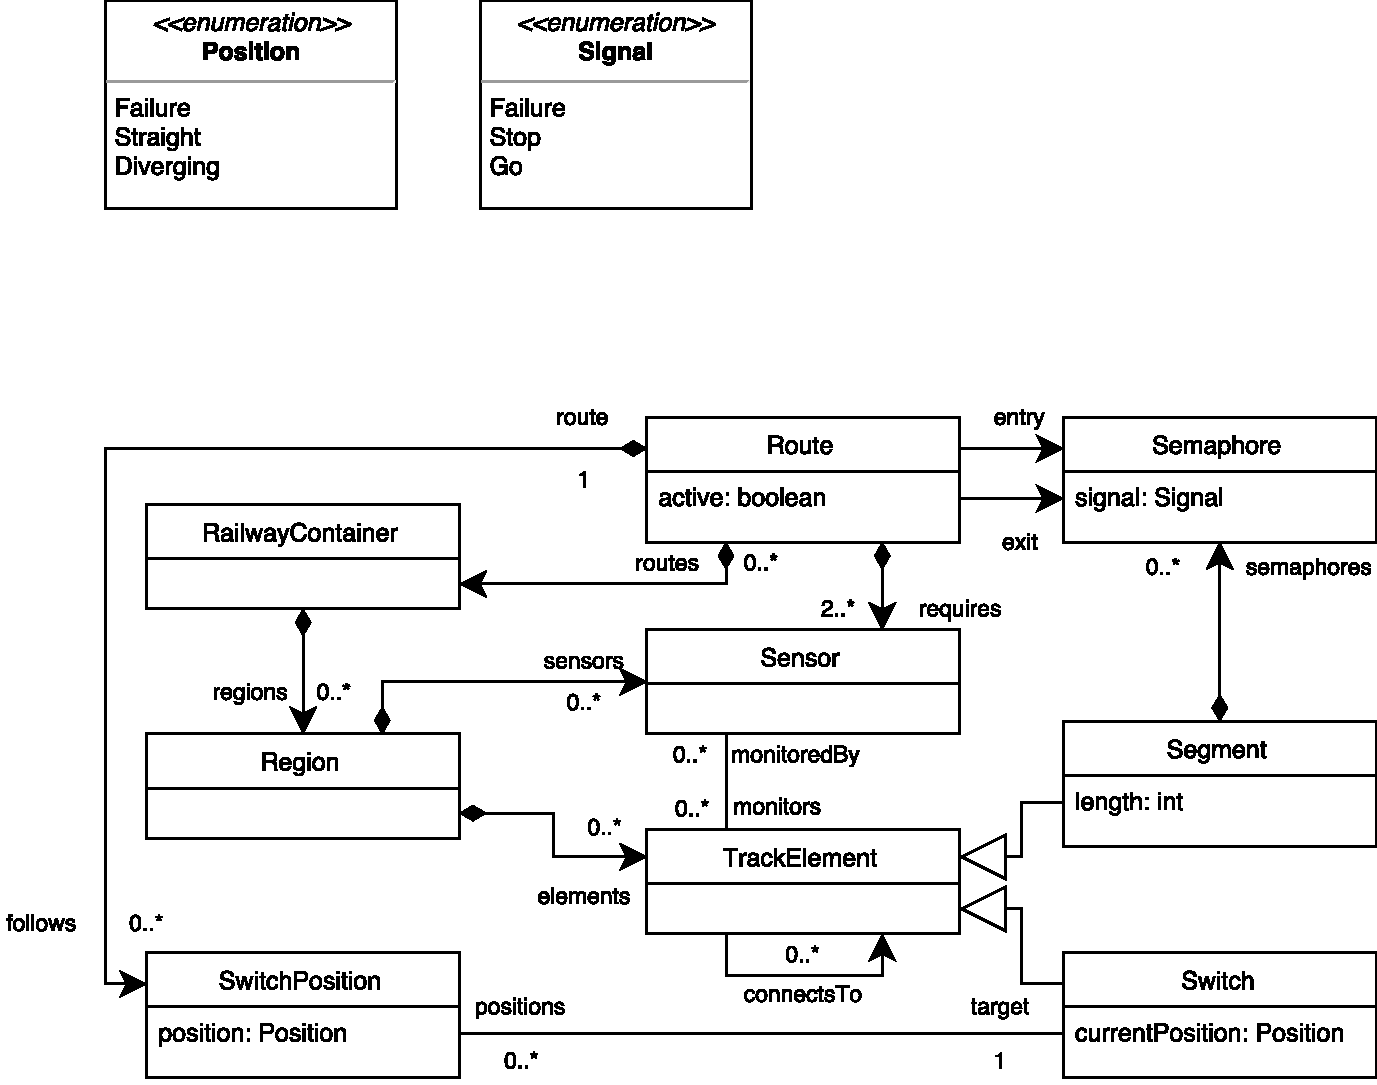
\includegraphics[width=\linewidth, keepaspectratio]{figures/model.pdf}
	\caption{A Train Benchmark modellje}
	\label{fig:ModelDiagram}
\end{figure}

\section{Kényszerek}

Erre a metamodellre számtalan kényszert meg lehetne követelni úgy, hogy még mindig lehessen olyan modellt alkotni, ami észszerűen nem felelhet meg a valóságnak. A Train Benchmarkban ezért csak összesen 6 kényszer teljesülését követelik meg. Ezek között vannak olyan egyszerűek, mint a \emph{PosLength}, ami azt követeli meg, hogy egy szegmens hossza pozitív legyen, és vannak bonyolultabbak, mint a \emph{ConnectedSegment}, ami azt, hogy 6 egymást követő szegmenst ne felügyeljen egy szenzor. Könnyen belátható, hogy ez utóbbi ellenőrzése egy relációs adatbázisban 7 tábla összekapcsolását követeli meg.

Két kényszert valósítottunk meg, ezért ezt a kettőt mutatnám be részletesebben.

\subsection{\emph{RouteSensor}}

Az utak és a rajtuk található váltók között nincs közvetlen kapcsolat. Az utakhoz csak a \emph{SwitchPosition} kapcsolódik, egy \emph{SwitchPosition} pedig pontosan egy váltóhoz tartozik. Ezáltal, ha közvetve is, de egy úthoz a rajta található váltókat hozzá lehet rendelni. A \emph{RouteSensor} azt követeli meg, hogy az úton található váltókhoz ne tartozhasson érzékelő úgy, hogy az út és az érzékelő között ne legyen kapcsolat.

\begin{figure}[!ht]
	\centering
	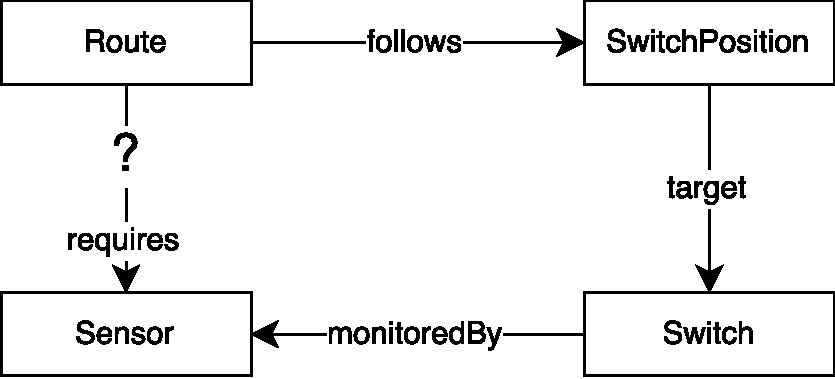
\includegraphics[width=0.7\linewidth, keepaspectratio]{figures/RouteSensor.pdf}
	\caption{A \emph{RouteSensor} kényszer}
	\label{fig:RouteSensor}
\end{figure}

\subsection{\emph{SwitchSet}}

A \emph{SwitchSet} kényszer teljesülésének feltétele, hogy amikor egy út aktív és az elején található szemafor szabad jelzést ad, akkor az összes váltónak olyan állásban kell lennie, hogy a vonat az adott úton haladjon végig.

\begin{figure}[!ht]
	\centering
	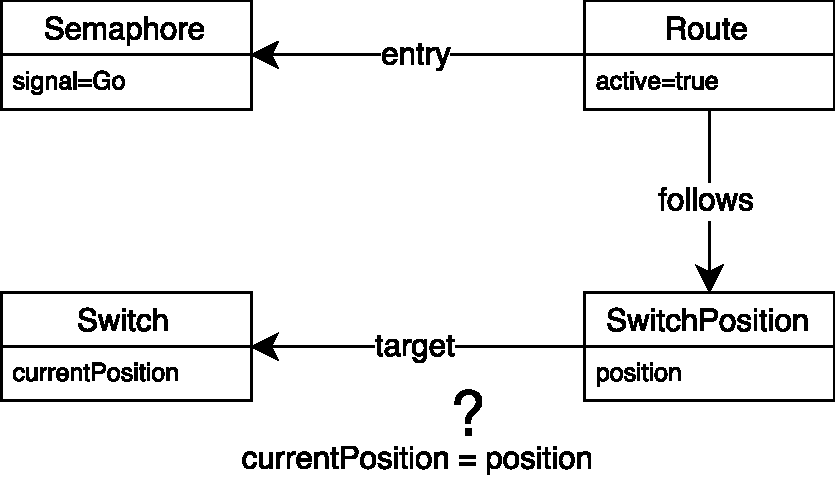
\includegraphics[width=0.7\linewidth, keepaspectratio]{figures/SwitchSet.pdf}
	\caption{A \emph{SwitchSet} kényszer}
	\label{fig:SwitchSet}
\end{figure}

%TODO Hiányzik innen egy bekezdés

\section{A fejlesztés lépései}

A valóságban egy ilyen modell folyamatosan bővül, azáltal, hogy új sínpályákat építenek, felújítják a régieket, az állomásokat. Ezáltal a számítógépes modellt is bővíteni kell, ami programozók feladata. Ilyen esetben előfordulnak hibák, amiket javítani kell. Ennek a szimulálására a Train Benchmark 3 különböző szcenáriót különböztet meg: \emph{Batch}, \emph{Inject}, \emph{Repair}.

\subsection{\emph{Batch}}

Ebben az esetben azt szimulálja a Train Benchmark, hogy az adatbázisba betöltenek egy modellt és ellenőrzik a kényszereket. Ez a fejlesztés első szakasza. A tesztelés célja mérni, hogy milyen gyorsan lehet egy már kész modellt importálni és a kényszereket először, mindenféle háttértudás nélkül ellenőrizni.

\subsection{\emph{Inject}}

Az \emph{Inject} szakaszban véletlenszerű hibainjektálás történik a modellbe és minden ilyen után egy újraellenőrzés következik. Ezáltal lehet mérni, ha egy modellben kis változtatásokat hajtanak végre, akkor az adott adatbázis-kezelő ezt mennyire ismeri fel, ezáltal képes-e a modell kis részét megváltoztatni és esetleg csak ezt újraellenőrizni. A hibainjektálás a különböző kényszerekhez más és más módon zajlik. A \emph{RouteSensor} megsértéséhez egy úthoz tartozó véletlenszerű \emph{requires} élet törlünk, a \emph{SwitchSet} megsértéséhez pedig a megfelelő váltó \emph{currentPosition} tulajdonságát érvénytelen értékre állítjuk.

\subsection{\emph{Repair}}

Ebben a fázisban a hibák kijavításának szimulálása zajlik. Itt is a javítást követően a kényszerek ismételt ellenőrzése következik. A javításhoz a hibabeszúráshoz képest általában sokkal több erőforrásra van szükség, mivel itt először meg is kell keresni a hibát, és csak utána lehet kijavítani. Ezt a \emph{RouteSensor} esetében  a hiányzó \emph{requires} él pótlásával, a \emph{SwitchSet} esetében a váltó \emph{currentPosition}-jének a \emph{SwitchPosition} \emph{position}-jéhez való igazításával lehet megtenni.

\section{\emph{Tool}-ok}

A Train Benchmark 10 különböző \emph{Tool}-ra, azaz adatbázis-kezelő szoftverre készült el. Ezek között található a napjainkban legelterjedtebb relációs adatbázis-kezelő, \emph{Eclipse Modeling Framework}-öt használó, illetve \emph{RDF}-alapú és gráfadatbázis is. A dolgozat ezek közül az \emph{RDF}-alapú Jena és  RDF4J futtatását követelte meg, így ezeket emelném ki. Az \emph{RDF} egy egyszerű gráfmodell leíró nyelv adatok közlésére a világhálón. Nagy előnye, hogy akkor is összefűzhető két ilyen módon leírt modell, ha különböző sémára épülnek. Mindezt úgy teszi lehetővé, hogy adathármasokat (\emph{triple}) tárol, ami a következőkből épül fel:
\begin{itemize}
	\item \emph{subject}: Az adathármas alanya, rá vonatkozik a \emph{triple}-ben tárolt adat.
	\item \emph{predicate}: Tulajdonság, a \emph{subject} és az \emph{object} közötti kapcsolat típusát írja le.
	\item \emph{object}: A tulajdonság tárgya, leírhat egyszerű tulajdonságot is, de amennyiben a predicate két, a modellben szereplő elem kapcsolatának típusát jelöli, akkor egy másik modellbeli elemet fog jelenteni.
\end{itemize}

\emph{Subject}, \emph{predicate}, \emph{object} hármas lehet a következő: \emph{Magyarország}, \emph{tengerpart}, \emph{nincs}; míg lehet az is, hogy \emph{Magyarország}, \emph{szomszéd}, \emph{Ausztria}. Míg az első esetben a predicate egy tulajdonságot jelölt, a második esetben egy kapcsolatot egy másik hasonló elemmel.

Az \emph{RDF4J}-ben és a \emph{Jena}-ban az a közös, hogy mindkettő egy Java keretrendszer \emph{rdf} alapú adatok feldolgozására, lekérdezésére és módosítására. Mindkettő \emph{SPARQL} lekérdező nyelvet használ.